\documentclass[12pt,a4paper]{article}
\usepackage[utf8]{inputenc}
\usepackage[spanish]{babel}
\usepackage[T1]{fontenc}
\usepackage{tocbibind} % Bibliografía en el indice
\usepackage{titlesec} % Posibilidad de editar los formatos de chapter
\usepackage{amsmath,amssymb,mathrsfs} % Matemáticas varias
\usepackage{siunitx} % SI de medidas
\usepackage{tabularx} % Para las tablas
\usepackage[title]{appendix} % Para anexos
\usepackage[spanish]{babel} % Para modificar labels por defecto
\renewcommand{\baselinestretch}{1} % Interlineado. 1 es estandar
% --- Arreglos varios para la inclusion de imagenes
\usepackage{float}
\usepackage[pdftex]{graphicx}
\usepackage{subfigure}
\usepackage{graphicx}
\graphicspath{{T:/Tom/Facultad/Logos/}{T:/Tom/Facultad/Materias/EDII/TPs/TPFinal/Diagramas/}}
\usepackage[usenames,dvipsnames]{color}
\DeclareGraphicsExtensions{.png,.jpg,.pdf,.mps,.gif,.bmp}
% --- Para las dimensiones de los márgenes etc
\frenchspacing \addtolength{\hoffset}{-1.5cm}
\addtolength{\textwidth}{3cm} \addtolength{\voffset}{-2.5cm}
\addtolength{\textheight}{4cm}
% --- Para el encabezado
\setlength{\headheight}{33pt}
\usepackage{fancyhdr}
\fancyhead[R]{\includegraphics[height=1cm]{logo_fcefyn_nuevo.jpg}}\fancyhead[L]{\includegraphics[height=1cm]{unc1_a.jpg}}\fancyhead[C]{Electrónica Digital II} \fancyfoot[C]{Página \thepage} \renewcommand{\footrulewidth}{0.4pt}
\pagestyle{fancy}
% --- Para las tablas
\usepackage{multirow} % Juntar filas
\newcolumntype{L}[1]{>{\raggedright\arraybackslash}p{#1}} % Justificar Izq
\newcolumntype{C}[1]{>{\centering\arraybackslash}p{#1}} % Justificar Centrar
\newcolumntype{R}[1]{>{\raggedleft\arraybackslash}p{#1}} % Justificar Der
\usepackage[numbered]{bookmark} % Para que figure las secciones en el PDF
\usepackage{listings} % Para poner código 
\usepackage{enumitem} % Para editar las propiedades de los items
\usepackage{color}
\usepackage[bottom]{footmisc} % Para las notas al pie de la página
\lstset{frame=single} % Código en un cuadro
% --- Para Anexo
\addto\captionsspanish{%
  \renewcommand\appendixname{ANEXO}
  \renewcommand\appendixpagename{ANEXOS}
}
% USar align sin numeracion y poner numeros donde quiera
\newcommand\numberthis{\addtocounter{equation}{1}\tag{\theequation}} 
% -------------------------------------------------------- %
% Definicion de colores para el codigo
\lstdefinelanguage{XML}
{
  basicstyle=\ttfamily\footnotesize,
  morestring=[b]",
  moredelim=[s][\bfseries\color{Maroon}]{<}{\ },
  moredelim=[s][\bfseries\color{Maroon}]{</}{>},
  moredelim=[l][\bfseries\color{Maroon}]{/>},
  moredelim=[l][\bfseries\color{Maroon}]{>},
  morecomment=[s]{<?}{?>},
  morecomment=[s]{<!--}{-->},
  commentstyle=\color{DarkOliveGreen},
  stringstyle=\color{blue},
  identifierstyle=\color{red}
}

\renewcommand{\lstlistingname}{Código}

% -------------------------------------------------------- %

\begin{document}

\begin{titlepage}
    \begin{center}
        \vspace*{1cm}
        
        \Large
        \textbf{Universidad Nacional de Córdoba\\
        		Facultad de Ciencias Exatas, Físicas y Naturales}
        
        \vspace{0.5cm}
        \includegraphics[width=0.5\textwidth]{logo_caratula.png}
        
        \vspace{1.5cm}
        
        \textbf{Trabajo Práctico Final}\\
        Electrónica Digital II\\
        Docente: Ing. Martín Del Barco
        
        \vfill  
        
        \vspace{0.8cm}
        

        
        \Large
        Losano Quintana, Juan Cruz\\
        Piñero, Tomás Santiago\\
        Ingeniería en Computación\\
        Año 2019\\
        
        
    \end{center}
\end{titlepage}
% -------------------------------------------------------- %

% --- Tabla de contenidos

\setcounter{secnumdepth}{1}
\setcounter{tocdepth}{4}
\tableofcontents

% -------------------------------------------------------- %

\newpage
\renewcommand{\baselinestretch}{1}
\setlength{\parskip}{0.5em}

\section{Introducción}
	Este informe trata sobre el trabajo práctico final de la materia Electrónica Digital II. El tema es a elección de los estudiantes, por lo que se eligió realizar un sensor de temperatura para propósitos generales.
	
\subsection{Enunciado}
	El sistema a realizar consiste en sensar la temperatura ambiente. La medición comienza cuando se presiona un botón. Una vez presionado se muestra el valor sensado en 4 (cuatro) \emph{displays} de siete segmentos con el formato ``XX$^{\circ}$C'' y se realiza un \emph{log} en la computadora cada cinco segundos.
	
	Para su realización se utilizaron los siguientes materiales:
	
	\begin{itemize}[leftmargin=1.5cm,nosep]
	\item Microcontrolador PIC16F887,
	\item Cristal de \SI{4}{\MHz},
	\item \emph{Bridge USB to UART} CP2102,
	\item Sensor de temperatura LM35,
	\item Cuatro \emph{displays} de siete segmentos cátodo común,
	\item Once transistores NPN XXXX,
	\item Resistencias de \SI{1}{\kilo\ohm}, \SI{330}{\ohm} y \SI{220}{\ohm},
	\item Capacitor de \SI{22}{\pico\F},
	\item Un pulsador.
	\end{itemize}

\section{Desarrollo}
		
\subsection{Cálculos realizados}

\subsubsection{Resistencias para los segmentos}
	El color de los \emph{displays} es rojo, por lo que cada segmento consume 1.7 [V] y 10 [mA], aproximadamente. Como la tensión de salida del PIC es $V_{OH} = 4.3\,[V]$, el cálculo queda:
	
	\begin{align*}
	algo &= 0\\
	R &= \frac{algo}{algomas}\\
	\\R &= 330 \, [\Omega] \numberthis
	\end{align*}
	
\newpage	
\subsubsection{Resistencias para la multiplexación}	
	Al tratarse de \emph{displays} de cátodo común, se necesitan transistores NPN para su multiplexación.
	
	La multiplexación consiste en encender un \emph{display} por vez, por lo que se necesita una frecuencia en la que el ojo sea capaz de ver \emph{todos} los \emph{displays} encendidos al mismo tiempo. Esta frecuencia es 50 [Hz].
	
	Por lo tanto, la fórmula para el tiempo \emph{t} de encendido de cada \emph{display} es la siguiente:

	\begin{equation}
	t = \frac{20\,[ms]}{N}
	\label{tiempo}
	\end{equation}
	
	 Siendo \emph{N} la cantidad de \emph{displays} a utilizar.
	 
	 Al tratase de cuatro \emph{displays} la ecuación \ref{tiempo} queda:
	 
	 \begin{align*}
	 t &= \frac{20\,[ms]}{4}\\
	 \\t &= 5\,[ms] \numberthis
	 \end{align*}

	 
\section{Implementación}
	El PIC tiene como frecuencia de reloj un cristal de \SI{4}{\MHz}, por lo que el ciclo de instrucción se realiza con una frecuencia de \SI{1}{\MHz} debido a que cada 4 ciclos del reloj se realiza una instrucción. Esto se debe a que para ejecutar la instrucción indicada, el PIC debe ejecutar cuatro acciones: 
	
	\begin{enumerate}[leftmargin=1.5cm,nosep]
	\item Buscar la instrucción en la memoria principal.
	\item Decodificar la instrucción.
	\item Ejecutar la instrucción.
	\item Almacenar los resultados.
	\end{enumerate}
	
	Esto es importante para el cálculo de la subrutina de retardo, ya que depende de la frecuencia de reloj que se utilice.

\newpage
\subsection{Diagramas de flujo}
	En esta sección se muestran los diagramas de flujo del programa principal y las subrutinas que utiliza.
	
	\subsubsection{Programa principal}	
	
	\begin{figure}[H]
	\includegraphics[scale=0.5]{main.png}
	\centering
	\caption{Diagrama de flujo del programa.}
	\end{figure}		
	
	Primero se realiza la configuración de los puertos:
	
	\begin{itemize}
	\item Puerto A: A0 como entrada analógica.
	\item Puerto B: RB0 como entrada digital.
	\item Puerto C como salida digital.
	\item Puerto D como salida digital.
	\end{itemize}
	
	Una vez configurados los puertos se configuran los módulos a utilizar.
	
	\begin{itemize}
	\item \emph{Timer0}: (Diagrama \ref{TM0}) se utiliza para la multiplexación de los \emph{displays}, por lo que se lo configura en modo temporizador para contar los 5 [ms]. El tiempo máximo que puede contar el \emph{timer0} con el \emph{prescaler} en 256 y la frecuencia de máquina en 1 [MHz] es:
	
	\begin{align*}
	\label{tmr0}
	t &= (256 - precarga) * 256 * 1\,[\mu s] \numberthis \\
	t_{max} &= 256 * 256 * 1\,[\mu s]\\
	\\t_{max} &\approx 65\,[ms] \numberthis
	\end{align*}
	
	\newpage
	Por lo tanto, para 5 [ms] la ecuación \ref{tmr0} queda:
	
	\begin{align*}
	5\,[ms] &= (256 - precarga) * 256 * 1\,[\mu s]\\
	\\ precarga &= 256 - \frac{5\,[ms]}{256 * 1\,[\mu s]}\\
	\\ precarga &= 236 \numberthis
	\end{align*}
	
	\item \emph{Timer1}: (Diagrama \ref{TM1}) este módulo también se utiliza en modo contador ya que se encarga de contar los cinco segundos. Al cumplirse este tiempo, se realiza una nueva conversión, actualizando el valor sensado, y lo envía al puerto serie.
	
	El tiempo máximo que puede contar este \emph{timer} con el \emph{prescaler} en 8 y la frecuencia de máquina en 1 [MHz] es:
	
	\begin{align*}
	\label{tmr1}
	t &= (65536 - precarga) * 8 * 1\,[\mu s]\\
	t_{max} &= 65536 * 8 * 1\,[\mu s]\\
	\\t_{max} &\approx 524\,[ms] \numberthis
	\end{align*}
	\end{itemize}
	
	Al no poder alcanzar los cinco segundos, se utiliza el \emph{timer1} para contar 500 [ms] y una variable auxiliar que se encargue de verificar que el \emph{timer1} se haya desbordado diez veces, consiguiendo así los cinco segundos necesarios. Para contar los 
	Consecuentemente, la ecuación \ref{tmr1} queda, para 500 [ms]:
	
	\begin{align*}
	500\,[ms] &= (65536 - precarga) * 8 * 1\,[\mu s]\\
	\\ precarga &= 65536 - \frac{500\,[ms]}{8 * 1\,[\mu s]}\\
	\\ precarga &= 3036 \numberthis
	\end{align*}
	
	Esta precarga debe realizarse en dos registros distintos debido a que el \emph{timer1} es de 16 bits. La parte alta del registro (TMR1H) se precarga con un valor de 0x0B, mientras que la parte baja del registro (TMR1L) se precarga con un valor de 0xDC, formando así un total de 3060 en decimal y 0x0BDC en hexadecimal.	
	
	Por último se precarga el valor que de temperatura ``00$^{\circ}$C'' que mostrará el programa mostrará el valor hasta que se presione el botón conectado en RB0.
	
	\newpage
	\subsubsection{Interrupciones}
	En esta sección se verifica qué módulo realizó la interrupción.
	
	\begin{figure}[H]
	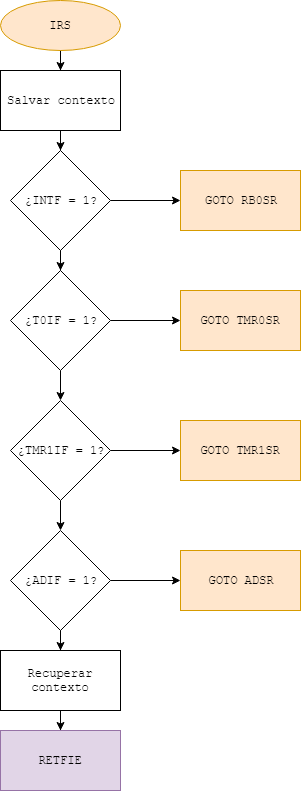
\includegraphics[scale=0.5]{IRS.png}
	\centering
	\caption{Diagrama de flujo de las interrupciones.}
	\label{IRS}
	\end{figure}		
	
	\newpage
	\paragraph{Interrupción por RB0} Esta interrupción inicia la conversión de la señal analógica que ingresa por A0.
	
	\begin{figure}[H]
	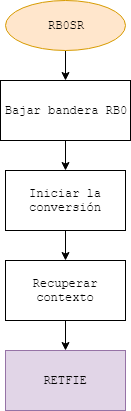
\includegraphics[scale=0.5]{RB0.png}
	\centering
	\caption{Diagrama de flujo de la interrupción por RB0.}
	\label{RB0}
	\end{figure}
	
	\paragraph{Interrupción por \emph{Timer0}} Si la interrupción es de \emph{timer0} se muestra el valor de la temperatura medida en los \emph{displays}.
	
	\begin{figure}[H]
	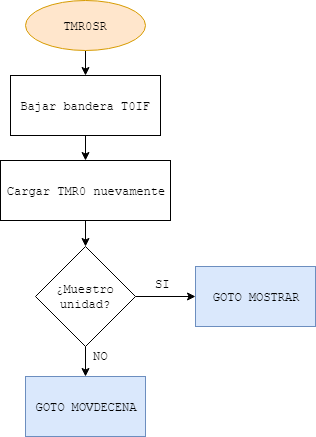
\includegraphics[scale=0.5]{TMR0.png}
	\centering
	\caption{Diagrama de flujo de la interrupción por \emph{Timer0}.}
	\label{TM0}
	\end{figure}
	
	\newpage
	\paragraph{Interrupción por \emph{Timer1}} Al desbordarse diez veces, habrán pasado los cinco segundos, por lo que se enviará el valor de la temperatura medida a la computadora y se iniciará una nueva conversión.
	
	\begin{figure}[H]
	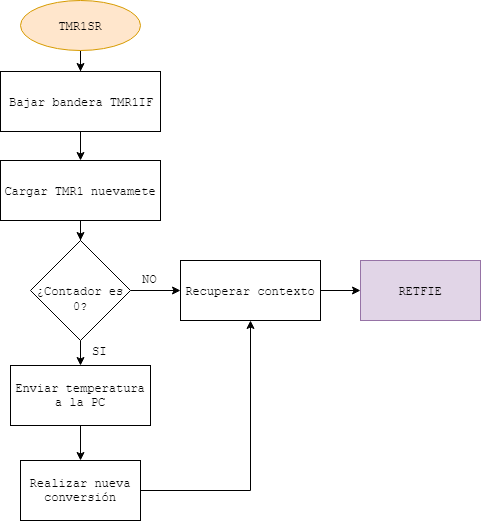
\includegraphics[scale=0.5]{TMR1.png}
	\centering
	\caption{Diagrama de flujo de la interrupción por \emph{Timer1}.}
	\label{TM1}
	\end{figure}
	
	\paragraph{Interrupción por \emph{ADC}} Si el conversor terminó la conversión de la señal, el resultado se rota hacia la izquierda para obtener el valor de temperatura medido y se actualiza el valor de la temperatura a mostrar. Para obtener el número de correspondiente a las decenas se resta 10 recursivamente al resultado obtenido hasta que dé negativo y luego se realiza el mismo proceso para la unidad, restando 1.
	
	\begin{figure}[H]
	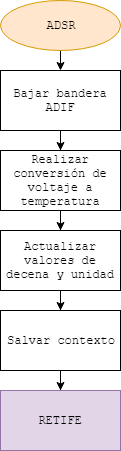
\includegraphics[scale=0.5]{ADC.png}
	\centering
	\caption{Diagrama de flujo de la interrupción por \emph{ADC}.}
	\label{ADC}
	\end{figure}
	
	\subsubsection{\emph{Delay}}
	Esta sub--rutina se encarga de darle al conversor los tiempos necesarios para la adquisición y conversión de los datos.
	
	El tiempo \emph{T} que demora este \emph{delay} es el siguiente:
	
	\begin{align*}
	T &= 4\, \mu s + 3\,\mu s * (DLAY - 1)\\
	T &= 4\, \mu s + 3\,\mu s * (250 - 1)\\
	\\T &= 751\, \mu s \numberthis
	\end{align*}
	
	\begin{figure}[H]
	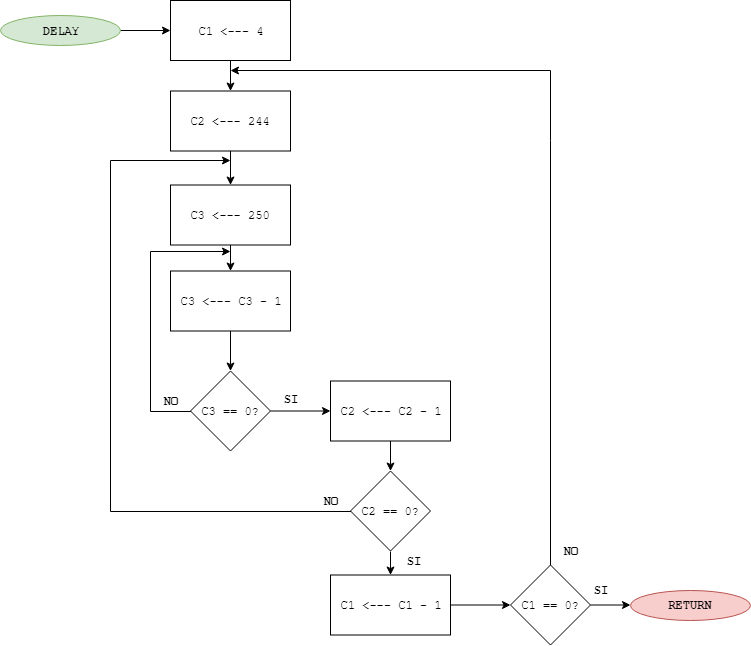
\includegraphics[scale=0.5]{delay.png}
	\centering
	\caption{Diagrama de flujo del \emph{delay}.}
	\end{figure}

\newpage
\section{Esquema del circuito}
\centering
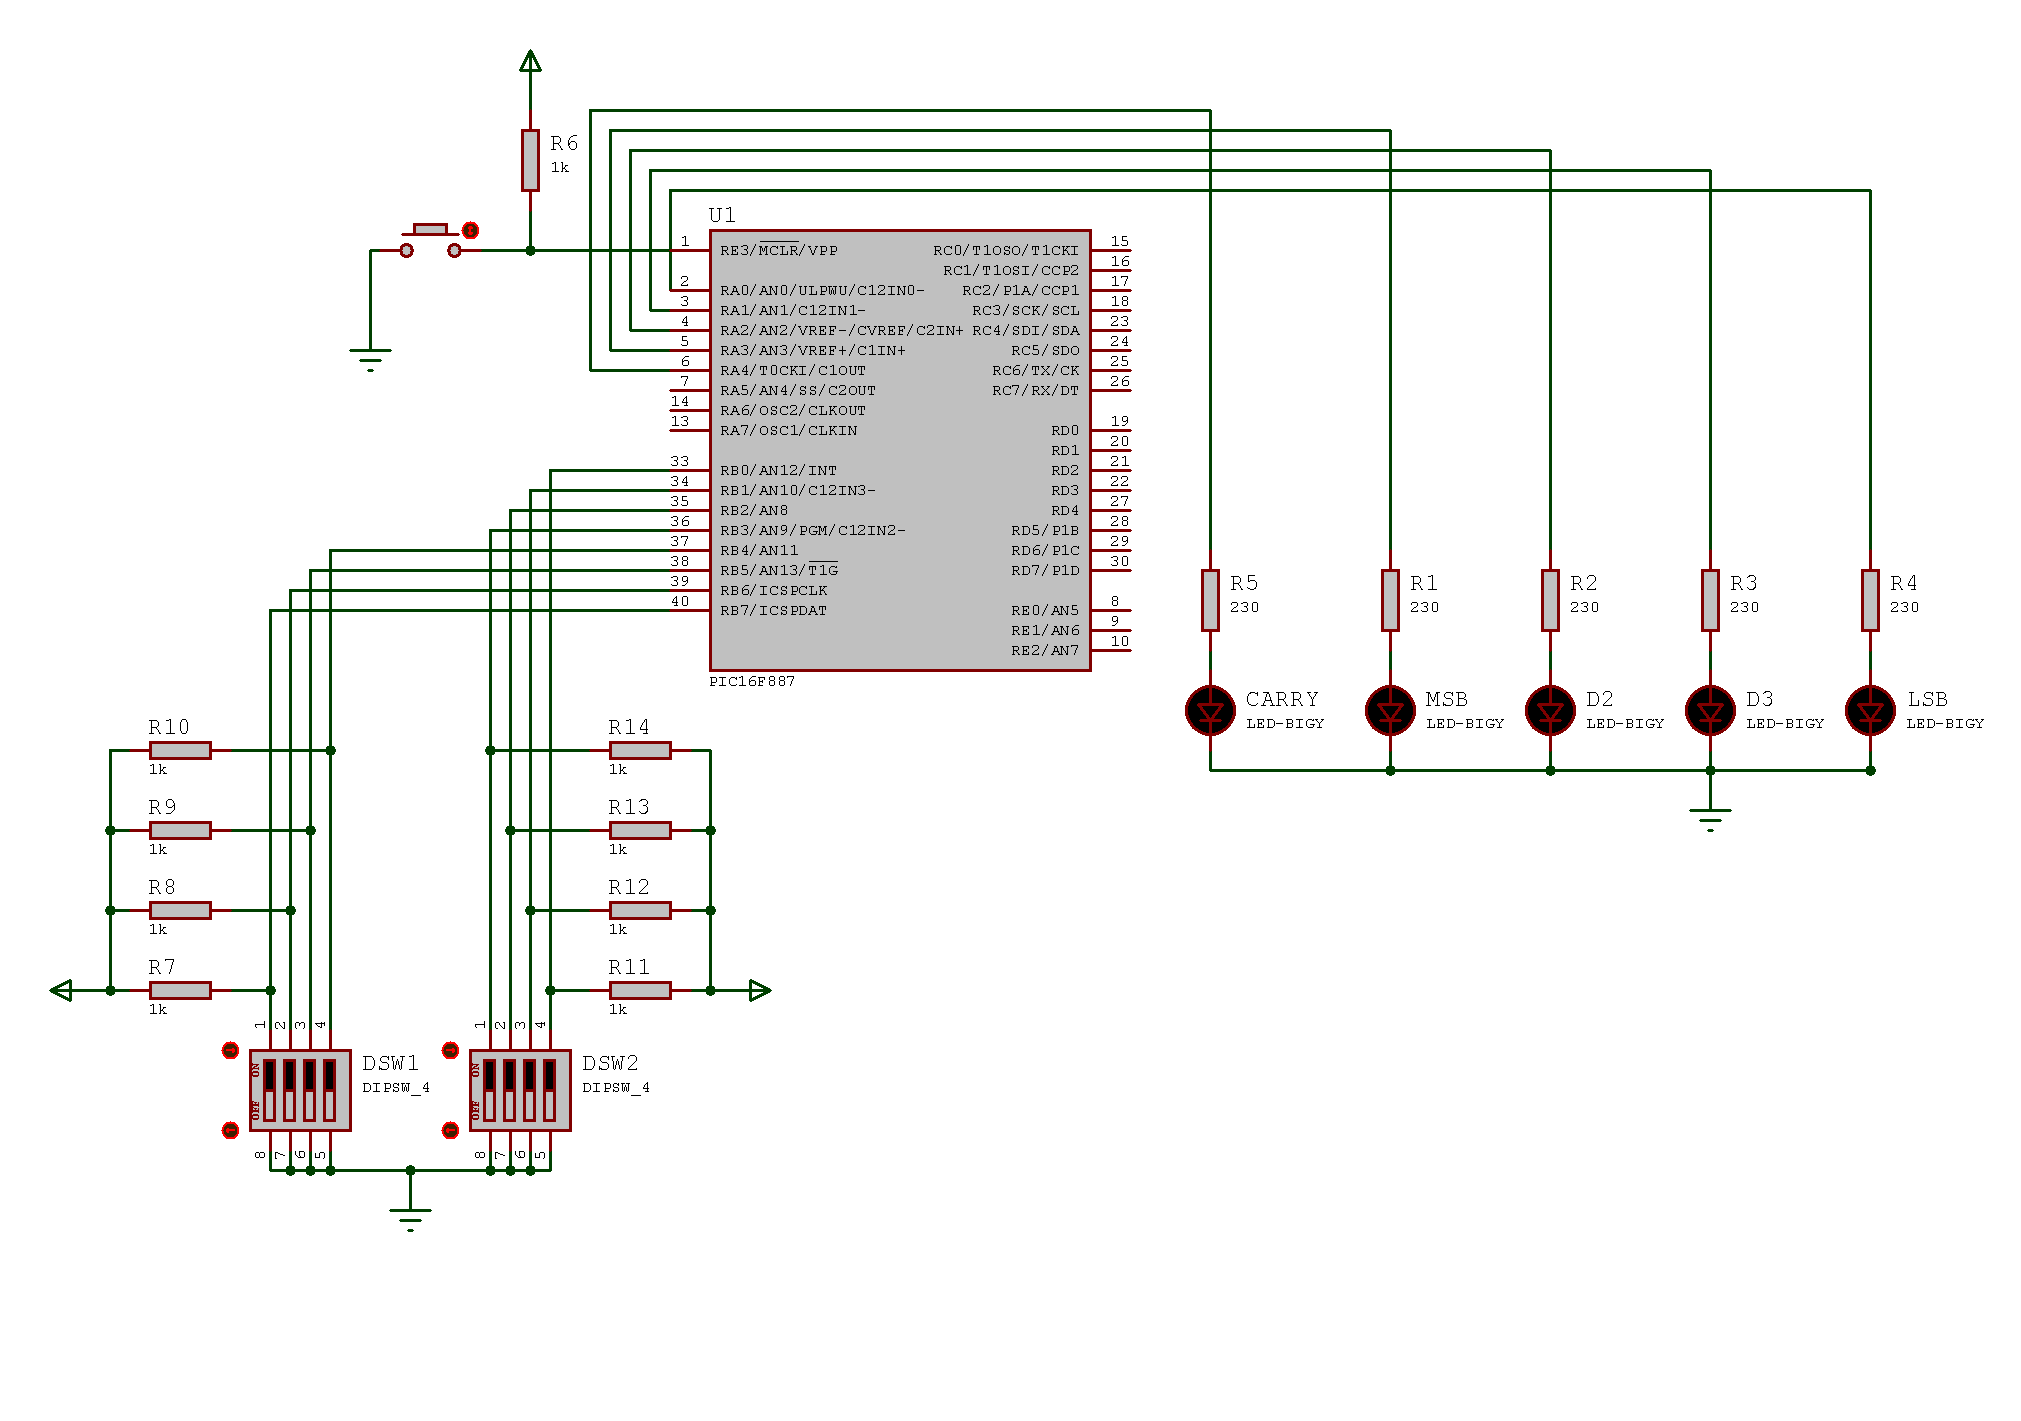
\includegraphics[angle=90,origin=c,scale=0.25]{circuito.png}
	
\end{document}